%% RiSE Latex Template - version 0.5
%%
%% RiSE's latex template for thesis and dissertations
%% http://risetemplate.sourceforge.net
%%
%% (c) 2012 Yguaratã Cerqueira Cavalcanti (yguarata@gmail.com)
%%          Vinicius Cardoso Garcia (vinicius.garcia@gmail.com)
%%
%% This document was initially based on UFPEThesis template, from Paulo Gustavo
%% S. Fonseca.
%%
%% ACKNOWLEDGEMENTS
%%
%% We would like to thanks the RiSE's researchers community, the 
%% students from Federal University of Pernambuco, and other users that have
%% been contributing to this projects with comments and patches.
%%
%% GENERAL INSTRUCTIONS
%%
%% We strongly recommend you to compile your documents using pdflatex command.
%% It is also recommend use the texlipse plugin for Eclipse to edit your documents.
%%
%% Options for \documentclass command:
%%         * Idiom
%%           pt   - Portguese (default)
%%           en   - English
%%
%%         * Text type
%%           bsc  - B.Sc. Thesis
%%           msc  - M.Sc. Thesis (default)
%%           qual - PHD qualification (not tested yet)
%%           prop - PHD proposal (not tested yet)
%%           phd  - PHD thesis
%%
%%         * Media
%%           scr  - to eletronic version (PDF) / see the users guide
%%
%%         * Pagination
%%           oneside - unique face press
%%           twoside - two faces press
%%
%%		   * Line spacing
%%           singlespacing  - the same as using \linespread{1}
%%           onehalfspacing - the same as using \linespread{1.3}
%%           doublespacing  - the same as using \linespread{1.6}
%%
%% Reference commands. Use the following commands to make references in your
%% text:
%%          \figref  -- for Figure reference
%%          \tabref  -- for Table reference
%%          \eqnref  -- for equation reference
%%          \chapref -- for chapter reference
%%          \secref  -- for section reference
%%          \appref  -- for appendix reference
%%          \axiref  -- for axiom reference
%%          \conjref -- for conjecture reference
%%          \defref  -- for definition reference
%%          \lemref  -- for lemma reference
%%          \theoref -- for theorem reference
%%          \corref  -- for corollary reference
%%          \propref -- for proprosition reference
%%          \pgref   -- for page reference
%%
%%          Example: See \chapref{chap:introduction}. It will produce 
%%                   'See Chapter 1', in case of English language.

\documentclass[pt,oneside,onehalfspacing,msc]{risethesis}

\usepackage[portuguese]{babel}
\usepackage{colortbl}
\usepackage{color}
\usepackage[table]{xcolor}
\usepackage{microtype}
\usepackage{bibentry}
\usepackage{subfigure}
\usepackage{multirow}
\usepackage{rotating}
\usepackage{booktabs}
\usepackage{pdfpages}
\usepackage{caption}
\usepackage{lipsum}
\usepackage{acronym}
\usepackage{amsfonts}
\usepackage{tabularx}
\usepackage{etoolbox}
\usepackage{algorithm}
\usepackage{tikz}
\usepackage{algpseudocode}
\usepackage{verbatim}

\usetikzlibrary{arrows,shapes}
\makeatletter

\addto\captionsportuguese{\renewcommand{\tablename}{Quadro}}
\AfterEndEnvironment{algorithm}{\let\@algcomment\relax}
\AtEndEnvironment{algorithm}{\kern2pt\hrule\relax\vskip3pt\@algcomment}
\let\@algcomment\relax
\newcommand\algcomment[1]{\def\@algcomment{\footnotesize#1}}

\renewcommand\fs@ruled{\def\@fs@cfont{\bfseries}\let\@fs@capt\floatc@ruled
	\def\@fs@pre{\hrule height.8pt depth0pt \kern2pt}%
	\def\@fs@post{}%
	\def\@fs@mid{\kern2pt\hrule\kern2pt}%
	\let\@fs@iftopcapt\iftrue}

\renewcommand{\ALG@name}{Pseudocódigo}
\renewcommand{\listalgorithmname}{Lista de \ALG@name s}
\algrenewcommand\algorithmicprocedure{\textbf{Procedimento}}
\algrenewcommand\algorithmicrepeat{\textbf{Repita}}
\algrenewcommand\algorithmicuntil{\textbf{Até que}}
\algrenewcommand\algorithmicfor{\textbf{Para}}
\algrenewcommand\algorithmicwhile{\textbf{Enquanto}}
\algrenewcommand\algorithmicdo{\textbf{Faça}}
\algrenewcommand\algorithmicif{\textbf{Se}}
\algrenewcommand\algorithmicelse{\textbf{Senão}}
\algrenewcommand\algorithmicthen{\textbf{Então}}
\algrenewtext{EndProcedure}{\textbf{Fim}}
\algrenewtext{EndIf}{\textbf{Fim}}
\algrenewtext{EndFor}{\textbf{Fim}}
\algrenewtext{EndWhile}{\textbf{Fim}}
\makeatother

\captionsetup[table]{position=top,justification=centering,width=.85\textwidth,labelfont=bf,font=small}
\captionsetup[lstlisting]{position=top,justification=centering,width=.85\textwidth,labelfont=bf,font=small}
\captionsetup[figure]{position=top,justification=centering,width=.85\textwidth,labelfont=bf,font=small}


%% Change the following pdf author attribute name to your name.
\usepackage[linkcolor=black,
            citecolor=blue,
            urlcolor=black,
            colorlinks,
            pdfpagelabels,
            pdftitle={Rise Thesis Template (ABNT)},
            pdfauthor={Rise Thesis Template (ABNT)}]{hyperref}

\address{RECIFE}

\universitypt{Universidade Federal Rural de Pernambuco}
\universityen{Federal Rural University of Pernambuco}

\departmentpt{Departamento de Estatística e Informática}
\departmenten{Department of Statistics and Informatics}

\programpt{Programa de Pós Graduação em Informática Aplicada}
\programen{MSc in Computer Science}

\majorfieldpt{Informática Aplicada}
\majorfielden{Applied Informatics}

\title{Title}

\date{2018}

\author{Author}
\adviser{Adviser}
\coadviser{Co-Adviser}

% Macros (defines your own macros here, if needed)
\def\x{\checkmark}

\begin{document}

\frontmatter

\frontpage

\begin{fichacatalografica}
	\FakeFichaCatalografica % Comment this line when you have the correct file
	%     \includepdf{fig_ficha_catalografica.pdf} % Uncomment this
\end{fichacatalografica}

\presentationpage

\banca

\begin{dedicatory}
	Dedicatory
\end{dedicatory}

\acknowledgements
\input{agradecimentos}

\begin{epigraph}[]{Albert Einstein}
Not everything that counts can be counted, and not everything that can be counted counts.
\end{epigraph}

\resumo
% Escreva seu resumo no arquivo resumo.tex


\begin{keywords}
keywords
\end{keywords}

\abstract
% Write your abstract in a file called abstract.tex

\begin{keywords}
keywords
\end{keywords}

% List of figures
\listoffigures

% List of tables
\listoftables

% List of pseudocodes
\listofalgorithms

% List of acronyms
% Acronyms manual: http://linorg.usp.br/CTAN/macros/latex/contrib/acronym/acronym.pdf
\listofacronyms
\begin{acronym}[ACRONYM] 
% Change the word ACRONYM above to change the acronym column width.
% The column width is equals to the width of the word that you put.
% Read the manual about acronym package for more examples:
%   http://linorg.usp.br/CTAN/macros/latex/contrib/acronym/acronym.pdf
%\acro{afm}[AFM]{Alphabet Frequency Matrix}
%\acro{api}[API]{Application Programming Interface}
%\acro{arima}[ARIMA]{Auto-Regressive Integrated Moving Average}
%\acro{brn}[BRN]{Bug Report Network}
%\acro{bts}[BTS]{Bug Triage System}
%\acro{cas}[CAS]{Context-Aware Systems}
%\acro{ccb}[CCB]{Change Control Board}
%\acro{cr}[CR]{Change Request}
%\acro{cvs}[CVS]{Concurrent Version System}
%\acro{es}[ES]{Expert System}
%\acro{floss}[FLOSS]{Free/Libre Open Source Software}
%\acro{glr}[GLR]{Generalized Linear Regression}
%\acro{gqm}[GQM]{Goal Question Metric}
%\acro{html}[HTML]{HyperText Markup Language}
%\acro{ir}[IR]{Information Retrieval}
%\acro{irt}[IRT]{Recôncavo Institute of Technology}
%\acro{jdt}[JDT]{Jazz Duplicate Finder}
%\acro{lda}[LDA]{Latent Dirichlet Allocation}
%\acro{loc}[LOC]{Lines of Code}
%\acro{lsi}[LSI]{Latent Semantic Indexing}
%\acro{ms}[MS]{Mapping Study}
%\acro{msr}[MSR]{Mining Software Repositories}
%\acro{nlp}[NLP]{Natural Language Processing}
%\acro{promise}[PROMISE]{Predictive Models in Software Engineering}
%\acro{rbes}[RBES]{Rule-Based Expert System}
%\acro{rhel}[RHEL]{RedHat Enterprise Linux}
%\acro{saas}[SaaS]{Software as a Service}
%\acro{scm}[SCM]{Software Configuration Management}
%\acro{serpro}[SERPRO]{Brazilian Federal Organization for Data Processing}
%\acro{slr}[SLR]{Stepwise Linear Regression}
%\acro{slr}[SLR]{Systematic Literature Review}
%\acro{svd}[SVD]{Singular Value Decomposition}
%\acro{svm}[SVM]{Support Vector Machine}
%\acro{svn}[SVN]{Subversion}
%\acro{tfidf}[TF-IDF]{Term Frequency-Inverse Document Frequency}
%\acro{vsm}[VSM]{Vector Space Model}
%\acro{xp}[XP]{Extreming Programming}
\acro{tmap}[TMAP]{Timed Multiagent Patrolling}
%\acro{tsp}[TSP]{Problema do Caixeiro Viajante}
%\acro{tspm}[TSPM]{Problema do Caixeiro Viajante com Múltiplas Visitas}
%\acro{ea}[EA]{Algoritmo Evolucionário}
%\acro{aco}[ACO]{\textit{Ant Colony Optimization}}
%\acro{es}[ES]{Estratégia Evolucionária}
%\acro{de}[DE]{Evolução Diferencial}
%\acro{ga}[GA]{Algoritmo Genético}
%\acro{mqi}[MQI]{Média Quadrática dos Intervalos}
%\acro{mqin}[MQIN]{Média Quadrática dos Intervalos Normalizada}
\end{acronym}

% Summary (tables of contents)
\tableofcontents

\mainmatter

\chapter{Introdução}
\label{chp:intro}

\section{Motivação}

\section{Objetivos}

\section{Contribuições obtidas}

\section{Organização do trabalho}

This work is organized as follows. \chapref{chp:literatureReview} has a literature review...
\chapter{Definição do problema}
\label{chp:problem}

Na patrulha multiagente um conjunto de agentes homogêneos e autônomos $A$ é 
utilizado para patrulhar um determinado ambiente. O ambiente de patrulha é uma 
área finita com pontos de interesse e caminhos entre esses pontos por onde os 
agentes podem se locomover, tal ambiente pode ser definido formalmente por um 
grafo não direcionado $G = (N, E)$, onde $N$ é o conjunto de vértices 
representando os pontos de interesse da área de patrulha e $E$ é o conjunto de 
arestas do grafo, o qual representa os caminhos entre os pontos do ambiente. 
Outras possíveis informações estáticas e úteis sobre o ambiente podem ser 
definidas como pesos nos vértices ou arestas do grafo $G$, a distância entre os 
pontos, por exemplo, é uma informação bastante útil e que pode ser definida como 
o peso das arestas. Os pesos dos vértices, por sua vez, podem ser utilizados 
para informar à estratégia de patrulha sobre pontos de maior importância, que 
demandam visitas mais periódicas. 

De acordo com uma estratégia de patrulha $S$ os agentes percorrem o ambiente, 
visitando os pontos de interesse continuamente durante o tempo $T$. Os instantes 
de visitas feitas pelos agentes em cada ponto são utilizados para calcular 
alguma métrica de patrulha $M$. A métrica de patrulha serve como medida de 
desempenho e pode ser calculada de modo a refletir diferentes aplicações e 
objetivos de patrulha.

Neste trabalho estamos interessados em considerar a patrulha multiagente com 
restrições na capacidade de comunicação dos agentes patrulhadores. A comunicação 
entre agentes é definida pela estratégia de patrulha, esta pode ser distribuída, 
onde a comunicação ocorre através de trocas de mensagens diretas entre os 
agentes; ou centralizada, onde uma base central de comunicações é responsável 
por receber todas as mensagens e por fazer a distribuição das mesmas, 
enviando-as para os destinatários. 

A forma de comunicação distribuída é mais suscetível à falhas devido à sua 
natureza dinâmica. Os agentes de patrulha estarão se movendo pelo ambiente 
durante todo o tempo e por muitas vezes poderão se encontrar isolados, fora do 
alcance dos demais agentes. Além disso, tentar usar equipamentos de comunicação 
mais potentes não é exatamente uma solução devido à possíveis limitações de 
consumo de energia do agente. 

Podemos modelar a restrição de comunicação como o raio de alcance máximo do 
equipamento de comunicação utilizado pelos agentes. Como já definido, assumimos 
agentes homogêneos, portanto todos devem possuir o mesmo alcance. Definimos a 
cobertura de comunicação de um agente como um círculo de raio máximo $r$ que se 
move juntamente com o agente e tem como centro a localização atual do mesmo no 
ambiente. Esta cobertura define o alcance de comunicação de cada agente durante 
a execução da patrulha onde, um agente fora da cobertura de outros está 
totalmente incapacitado de se comunicar com os demais; para agentes que se 
encontram dentro da área de cobertura de outros agentes a chance da comunicação 
acontecer com sucesso é inversamente proporcional à distância que os agentes se 
encontram um do outro.

\chapter{Revisão da Literatura}
\label{chp:literatureReview}


\chapter{Conclusões e Trabalhos Futuros}
\label{conclusion}

\section{Trabalhos Futuros}

\chapter{Examples}
\label{chp:ex}

\begin{figure}[tp]
	\caption[Example]{Example}
	\centering
	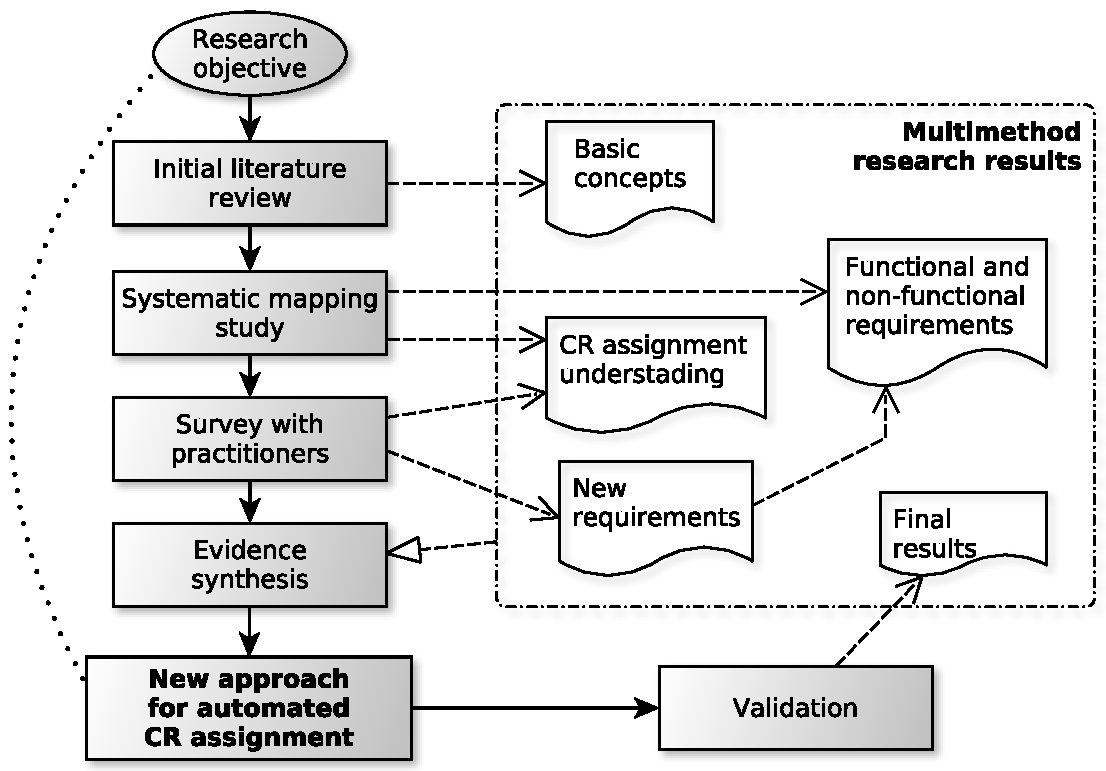
\includegraphics[width=0.75\columnwidth]{images/img1.pdf}
	\caption*{Fonte: \citep{einstein1907252}}
	\label{fig:graphexample}
\end{figure}

\begin{table}[bh]
	\centering
	\caption{Resumo dos operadores apresentados}
	\label{tbl:resumo_operadores}
	\begin{tabularx}{\linewidth}{|X|X|X|}
		\hline
		\textbf{Operador} & \textbf{Operação} & \textbf{Referência} \\
		\hline
		\textit{Random Centering} & Criação de Indivíduos & Proposto neste trabalho \\
		\hline
		\textit{Approximated Maximum Distance Centering} & Criação de Indivíduos & Proposto neste trabalho \\
		\hline
		\textit{Random Partitioning} & Criação de Indivíduos & Proposto neste trabalho \\
		\hline
		\textit{Heuristic Graph Partitioning} & Criação de Indivíduos & Proposto neste trabalho \\
		\hline
		\textit{Random Path Building} & Criação de Indivíduos & Proposto neste trabalho \\
		\hline
		\textit{Nearest Neighbor Path Building} & Criação de Indivíduos & EXAMPLE \\
		\hline
		\textit{Nearest Insertion Path Building} & Criação de Indivíduos & EXAMPLE \\
		\hline
		Melhorar & Mutação & Proposto neste trabalho \\
		\hline
		\textit{2-change} & Mutação & EXAMPLE \\
		\hline
		\textit{Half Add Half Sub Small Changes} & Mutação & Proposto neste trabalho \\
		\hline
		\textit{Half Add Half Sub Rebuild} & Mutação & Proposto neste trabalho \\
		\hline
		\textit{Simple Random Crossover} & Recombinação & Proposto neste trabalho \\
		\hline
	\end{tabularx}
	\caption*{Fonte: O autor}
\end{table}


\begin{algorithm}                  % enter the algorithm environment
	\caption{\textit{Heuristic Graph Partitioning}}          % give the algorithm a caption
	\label{partitioning_fungal}                           % and a label for \ref{} commands later in the document
	\algcomment{\begin{center} Fonte: O Autor \end{center}}
	\begin{algorithmic}[1]                    % enter the algorithmic environment
		\Procedure{GRAPH-PARTITIONING}{$centros, G(V,E)$}
		\newline
		\Comment{$G$ é o o grafo e $centros$ é a lista de centros calculados anteriormente}
		\State $ParticaoPorVertice \gets $ \{\}
		\State $ListaDeVerticesPorCentro \gets $ \{\}
		\State $ParticaoDoCentro \gets $ \{\}
		\For{$i \in V$}
			\If{$i \in centros$}
				\State $ParticaoPorVertice[i] \gets i$
			\Else
				\State $ParticaoPorVertice[i] \gets -1$
			\EndIf
		\EndFor
		\For{$centro \in centros$}
			\State $ListaDeVerticesPorCentro(centro) \gets $ lista dos nós do grafo ordenados pelas suas distâncias ao $centro$
			\State $ParticaoDoCentro(centro) \gets $ \{\}
		\EndFor
		\Repeat
			\For{$C_{i} \in centros$}
				\While{$ListaDeVerticesPorCentro(C_{i}) \neq \{\}$}
					\State $n \gets $ REMOVE-PRIMEIRO($ListaDeVerticesPorCentro(C_{i})$)
					\If{$ParticaoPorVertice(n) = -1$}
						\State $ParticaoPorVertice(n) \gets C_{i}$
						\State \textbf{Pare o Laço Enquanto}
					\EndIf
				\EndWhile
			\EndFor
		\Until{$-1 \notin ParticaoPorVertice$} \Comment{Até que todo vértice esteja em uma partição}
		\For{$v \in V$}
			\State $ParticaoDoCentro(ParticaoPorVertice(v)) \cup $ {o menor caminho entre ParticaoPorVertice(v) e v}
		\EndFor
		\State \textbf{Retorne} as partições em $ParticaoDoCentro$
		\EndProcedure
	\end{algorithmic}
\end{algorithm}

\tikzstyle{vertex}=[circle,fill=black!25,minimum size=20pt,inner sep=0pt]
\tikzstyle{red vertex}=[circle,fill=red!25,minimum size=20pt,inner sep=0pt]
\tikzstyle{green vertex}=[circle,fill=green!25,minimum size=20pt,inner sep=0pt]
\tikzstyle{green edge} = [draw,line width=2pt,-,green!50]
\tikzstyle{red edge} = [draw,line width=2pt,-,red!50]

\begin{figure}
	\caption{Exemplo de solução da \ac{tmap}}
	\centering
	\begin{tikzpicture}
	[scale=.8,auto=left,every node/.style={circle,fill=blue!20}]
	\node[vertex] (n6) at (1,6)  {6};
	\node[vertex] (n0) at (4,12) {0};
	\node[vertex] (n1) at (8,12) {1};
	\node[vertex] (n2) at (12,6) {2};
	\node[vertex] (n4) at (2,1)  {4};
	\node[red vertex] (n5) at (5,9)  {5};
	\node[vertex] (n7) at (10,1) {7};
	\node[green vertex] (n3) at (7,9)  {3};
	
	\foreach \from/\to in {n0/n6,n6/n4,n4/n5,n5/n0}
		\path[red edge] (\from) -- (\to);
	\foreach \source/\dest in {n1/n2,n2/n7,n7/n3,n3/n1}
		\path[green edge] (\source) -- (\dest);
	\foreach \de/\para in {n0/n1}
		\draw (\de) -- (\para);
	
	\end{tikzpicture}
	\caption*{Fonte: O autor}
	\label{fig:tmap_example}
\end{figure}


% References

\begin{references}
  \bibliography{references}
\end{references}

% Appendix

%\theappendix
%\chapter{Mapping Study's Instruments}
\label{ap:mapping-study}

\begin{table}[!htp]
	\centering
	\caption{List of conferences on which the searches were performed.}
	\label{tbl:conferences_list}
	\rowcolors{2}{lightgray!30}{white}
	\resizebox{\columnwidth}{!}{
	\begin{tabular}{ll}
	\toprule
	\textbf{Acronym} & \textbf{Conference} \\
	\toprule
	APSEC & Asia Pacific Software Engineering Conference \\
	ASE   & IEEE/ACM International Conference on Automated Software Engineering \\
	CSMR  & European Conference on Software Maintenance and Reengineering \\
	ESEC  & European Software Engineering Conference \\
	ESEM  & International Symposium on Empirical Software Management and Measurement \\
	ICSE  & International Conference on Software Engineering \\
	ICSM  & International Conference on Software Maintenance \\
	ICST & International Conference on Software Testing \\
	InfoVis & IEEE Information Visualization Conference \\
	KDD   & ACM SIGKDD International Conference on Knowledge Discovery and Data Mining \\
	MSR   & Working Conference on Mining Software Repositories \\
	OOPSLA & Object-Oriented Programming, Systems, Languages and Applications \\
	QSIC  & International Conference On Quality Software \\
	SAC & ACM Symposium on Applied Computing \\
	SEAA & EUROMICRO Conference on Software Engineering and Advanced Applications\\
	SEDE & 19th International Conference on Software Engineering and Data Engineering \\
	SEKE  & International Conference on Software Engineering and Knowledge Engineering \\
	\bottomrule
	\end{tabular}
	}
\end{table}

\begin{table}[htp]
	\caption{List of journals in which the searches were performed.}
	\label{tbl:journals_list}
	\centering
	\rowcolors{2}{lightgray!30}{white}
	\begin{tabular}{l}
	\toprule
	\textbf{Journal title} \\
	\toprule
	ACM Transactions on Software Engineering and Methodology \\
	Automated Software Engineering \\
	Elsevier Information and Software Technology \\
	Elsevier Journal of Systems and Software \\
	Empirical Software Engineering \\
	IEEE Software \\
	IEEE Computer \\
	IEEE Transactions on Software Engineering \\
	International Journal of Software Engineering and Knowledge Engineering \\
	Journal of Software: Evolution and Process \\
	Software Quality Journal \\
	Journal of Software \\
	Software Practice and Experience Journal \\
	\bottomrule
	\end{tabular}
\end{table}

\begin{table}[h]
\centering
\footnotesize
 \rowcolors{2}{lightgray!30}{white}
\caption{Search string per Search Engine.}
\label{tbl:stringengine}
\begin{tabular}{p{.15\textwidth}p{.8\textwidth}}
\toprule
\textbf{Search Engine} & \textbf{Search String}\\
\toprule
   	 	Google Scholar &  bug report OR track OR triage ``change
   	 	request'' issue track OR request OR software OR ``modification request'' OR
   	 	``defect track'' OR ``software issue''  repositories maintenance evolution\\

   	 	ACM Portal & Abstract: "bug report" or Abstract:"change request"
   	 	or Abstract:"bug track" or Abstract:"issue track" or  Abstract:"defect
   	 	track" or Abstract:"bug triage" or Abstract: "software issue" or Abstract: "issue request"
   	 	or Abstract: "modification request") and  (Abstract:software or
   	 	Abstract:maintenance or Abstract:repositories or Abstract:repository \\

   	 	IEEExplorer (1) & (((((((((("Abstract": "bug report") OR
   	 	"Abstract":"change request") OR "Abstract":"bug track") OR "Abstract":"software issue") OR "Abstract":"issue request") OR
        "Abstract":"modification request") OR "Abstract":"issue track") OR
	    "Abstract":"defect track") OR "Abstract":"bug triage") AND
	    "Abstract":software)\\

         IEEExplorer (2) & (((((((((("Abstract": "bug report") OR
         "Abstract":"change request") OR "Abstract":"bug track") OR "Abstract":"software issue") OR
         "Abstract":"issue request") OR "Abstract":"modification request") OR
         "Abstract":"issue track") OR "Abstract":"defect track") OR
         "Abstract":"bug triage") AND "Abstract":maintenance)\\

         IEEExplorer (3) & (((((((((("Abstract": "bug report") OR
         "Abstract":"change request") OR "Abstract":"bug track") OR "Abstract":"software issue") OR
         "Abstract":"issue request") OR "Abstract":"modification request") OR
         "Abstract":"issue track") OR "Abstract":"defect track") OR
         "Abstract":"bug triage") AND "Abstract":repositories)\\

         IEEExplorer & (((((((((("Abstract": "bug report") OR
         "Abstract":"change request") OR "Abstract":"bug track") OR "Abstract":"software issue") OR
         "Abstract":"issue request") OR "Abstract":"modification request") OR
         "Abstract":"issue track") OR "Abstract":"defect track") OR
         "Abstract":"bug triage") AND "Abstract": repository)\\

         Citeseer Library & (abstract: "bug report" OR abstract:"change request" OR abstract:"bug track" OR abstract:"issue track" OR
	     abstract:"defect track" OR abstract:"bug triage" OR abstract: "software
	     issue" OR abstract: "issue request" OR abstract: "modification request")
	     AND (abstract:software OR abstract:maintenance OR abstract:repositories OR
	     abstract:repository)\\

	     Elsevier & ("bug report" OR "change
	     request" OR "bug track" OR "issue track" OR "defect track" OR "bug triage" OR "software issue" OR  "issue request" OR
	    "modification request") AND (software OR maintenance OR repositories OR
	    repository)\\

	    Scirus & ("bug report" OR "change request" OR "bug track" OR "issue track" OR  "defect track" OR "bug triage" OR
        "software issue" OR  "issue request" OR "modification request") AND
	    (software maintenance OR repositories OR repository) ANDNOT (medical OR
	    aerospace)\\

	    ScienceDirect & ("bug report" OR "change request" OR "bug track"
	     OR "issue track" OR "defect track" OR "bug triage" OR "issue request" OR
	     "modification request") AND LIMIT-TO(topics, "soft ware")\\

	     Scopus & ("bug report" OR "change request" OR "bug track" OR
	     "issue track" OR  "defect track" OR "bug triage" OR "software issue" OR
	     "issue request" OR "modification request") AND (software maintenance OR
	     repositories OR repository)\\

	     Wiley & ("bug report" OR "change request"
	     OR "bug track" OR "issue track" OR  "defect track" OR "bug triage" OR
         "software issue" OR  "issue request" OR "modification request") AND
	     (software maintenance OR repositories OR repository)\\

	     ISI Web\newline of Knowledge & ("bug report" OR "change request" OR "bug
	     track" OR "issue track" OR  "defect track" OR "bug triage" OR "software issue" OR  "issue request" OR "modification request") AND
	    (software maintenance OR repositories OR repository) ANDNOT (medical OR
	    aerospace)\\

	    SpringerLink & ("bug report" OR "change request" OR "bug track" OR "issue track" OR  "defect track" OR "bug triage" OR
        "software issue" OR  "issue request" OR "modification request") AND
	    (software maintenance OR repositories OR repository) ANDNOT (medical OR
	    aerospace)\\
	\bottomrule
\end{tabular}
\end{table}

\end{document}
